\documentclass{beamer}
\usetheme{metropolis}

\usepackage[T1]{fontenc}

\title{Kolorowania węzłów i niezmienniki homologiczne\\%
{\normalfont\small%
Praca napisana pod kierunkiem prof. dr hab. Tadeusza Januszkiewicza%
}%
}
\date{06.12.2024}

\author{Weronika Jakimowicz}
\institute{Instytut Matematyczny Uniwersytetu Wrocławskiego}

\usepackage{amssymb}
\usepackage{amsmath}
\usepackage{mathtools}
\usepackage{dsfont}

\usetikzlibrary{cd, patterns, patterns.meta, decorations.pathmorphing, calc, matrix, positioning, arrows, arrows.meta, spath3, hobby, knots, braids}

\DeclareMathOperator{\Z}{\mathbb{Z}}
\DeclareMathOperator{\R}{\mathbb{R}}
\DeclareMathOperator{\C}{\mathbb{C}}
\DeclareMathOperator{\N}{\mathbb{N}}
\DeclareMathOperator{\Q}{\mathbb{Q}}

\DeclareMathOperator{\coker}{coker}

\definecolor{green}{HTML}{859900}
\definecolor{white}{HTML}{fafafa}
\definecolor{bg}{HTML}{fafafa}

\newenvironment{deff}{\begin{block}{Definicja}}{\end{block}}

\pagestyle{empty}

% \usepackage[
%     backend=biber,
%     style=alphabetic,
%   ]{biblatex}

% \addbibresource{lit.bib}
 

\begin{document}\metroset{block=fill}
  \maketitle
  % \section{First Section}
  \begin{frame}{Węzeł i jego grupa}

    \begin{columns}[T,onlytextwidth]

      \column{.4\textwidth}

      \begin{deff}
        Węzeł to gładkie zanurzenie $S^1\hookrightarrow S^3$. 
      \end{deff}

      \column{.59\textwidth}

      \begin{deff}
        Niech $K\subseteq S^3$ będzie węzłem. Wtedy grupa $\pi_1(S^3-K)$ jest nazywana \textbf{grupą węzła} $K$.
      \end{deff}

    \end{columns}

      % \column{.5\textwidth}

      Rzutowanie $D:S^1\hookrightarrow \R^2$ węzła nazywa się \emph{diagramem}.
    
      \begin{figure}\centering\scalebox{0.8}{
    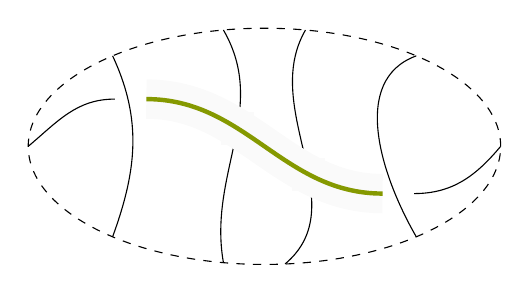
\begin{tikzpicture}
      \draw[name path=down1] ($(100:3 and 1.5)+(1.5, 0)$) to[out=-60, in=100] ($(1.5, 0)+(-100:3 and 1.5)$);
      \draw[name path=down2] ($(80:3 and 1.5)+(1.5, 0)$) to[out=-120, in=40] ($(1.5, 0)+(-85:3 and 1.5)$);
      
      \draw[line width=5mm, white, name path=to-be-green] (0, .6) to[out=0, in=180] (3, -.6);

      \path [name intersections={of=to-be-green and down1,by=D1}];
      \node [fill=bg,inner sep=6pt,label=-90:] at (D1) {};

      \path [name intersections={of=to-be-green and down2,by=D2}];
      \node [fill=bg,inner sep=6pt,label=-90:] at (D2) {};

      \draw (-.4, .6) to[out=180, in=40] (-1.5, 0);
      \draw (3.4, -.6) to[out=0, in=-130] (4.5, 0);

      \draw[ultra thick, green] (0, .6) to[out=0, in=180] (3, -.6);
      \draw ($(1.5,0)+(130:3 and 1.5)$) to[out=-65, in=70] ($(1.5,0)+(-130:3 and 1.5)$);
      \draw ($(1.5, 0)+(-50:3 and 1.5)$) to[out=120, in=200] ($(50:3 and 1.5)+(1.5, 0)$);

      \draw[dashed] (1.5, 0) ellipse(3 and 1.5);
  \end{tikzpicture}}
    \end{figure}

  \end{frame}

  \begin{frame}{Niezmienniki węzłów}
    \begin{itemize}
      \item Grupa węzła jest skomplikowana do wyliczenia. 
      \item Wielomian Alexandera liczymy m.in. z diagramu, ale nie zawsze jest pomocny, np:
    \end{itemize}
%
    \begin{columns}[T,onlytextwidth]
      \column{0.49\textwidth}
%
      \begin{figure}[h]\centering
          $K11n85$ 

        \scalebox{.3}{ 
    \begin{tikzpicture}
      \coordinate (a1) at (90:6);
      \coordinate (a2) at (0: 2);
      \coordinate (a3) at ($(-90:5.5)+(4, 0)$);
      \coordinate (a4) at (-80:2);
      \coordinate (a5) at (-90:5.5);
      \coordinate (a6) at (-10:5);
      \coordinate (a7) at (30:7);
      \coordinate (a8) at (180:2.5);
      \coordinate (a9) at (-90:3.5);
      \coordinate (a10) at (-10:7);
      \coordinate (a11) at (110:2);

      % \foreach \i in {1,..., 11} \fill (a\i) circle (5pt);

      \begin{knot}[
        consider self intersections, 
        clip width = 20pt,
        % draft mode=crossings, 
        ignore endpoint intersections=false,
        flip crossing=1, 
        flip crossing=3,
        flip crossing=4, 
        flip crossing=5, 
        flip crossing=7, 
        flip crossing=11, 
        flip crossing=12, 
        flip crossing=9
        ]
        \strand[thick] (a1) to[out=-30, in=90] 
        (a2) to[out=-90, in=200] 
        (a3) to[out=20, in=0, looseness=2]
        (a4) to[out=180, in=180, looseness=2] 
        (a5) to[out=0, in=-100] 
        (a6) to[out=80, in=-60] 
        (a7) to[out=120, in=90]
        (a8) to[out=-90, in=180] 
        (a9) to[out=0, in=-90, looseness=2] 
        (a10) to[out=90, in=0]
        (a11) to[out=180, in=150, looseness=1.5]
        (a1);
      \end{knot}
    \end{tikzpicture}
  }


    % \caption{A diagram for knot $K11n85$.\label{k11n85 diagram}}
  \end{figure}


  \column{.49\textwidth}

  \begin{figure}[h]\centering 
  $K11n164$

    \scalebox{.3}{
    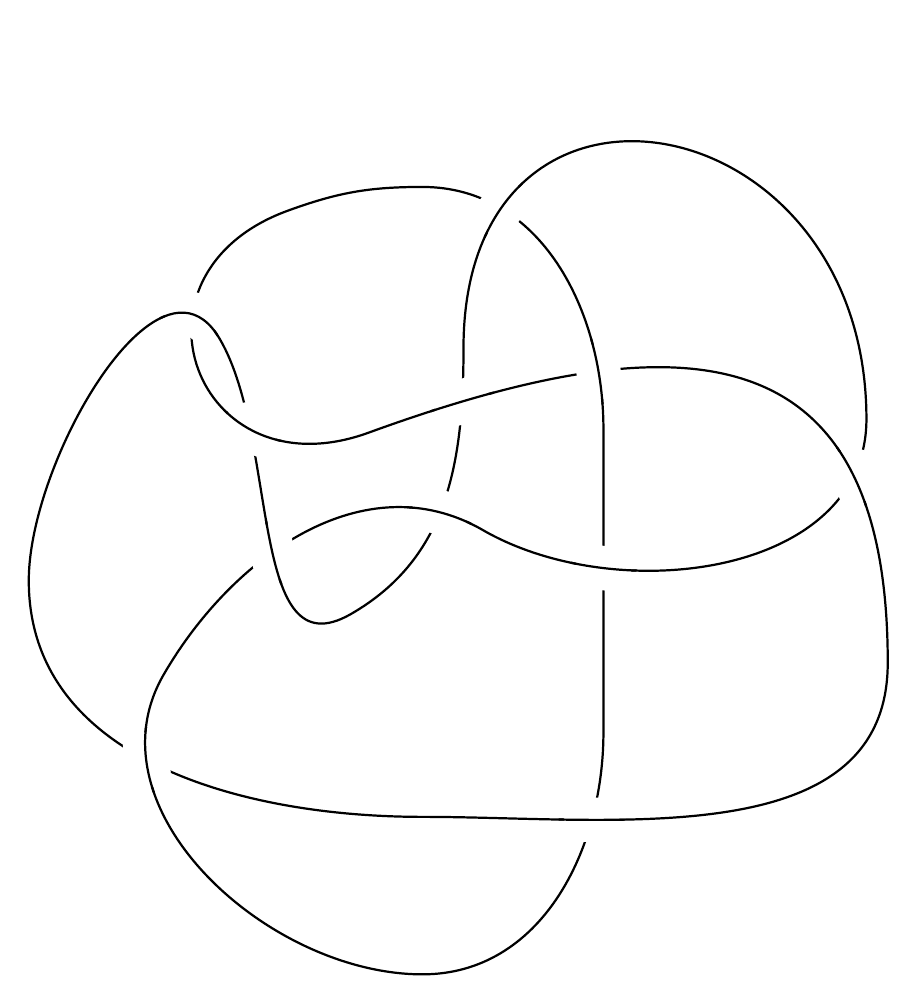
\begin{tikzpicture}
      \coordinate (a1) at (90:5);
      \coordinate (a2) at (40:3);
      \coordinate (a3) at (-40:3);
      \coordinate (a4) at (-90:5);
      \coordinate (a5) at (-160:3.5);
      \coordinate (a6) at (40:1);
      \coordinate (a7) at (20:6);
      \coordinate (a8) at (80:3);
      \coordinate (a9) at (180+25:1);
      \coordinate (a10) at (130:4);
      \coordinate (a11) at (180:5);
      \coordinate (a12) at (-90:3);
      \coordinate (a13) at (-10:6);
      \coordinate (a14) at (110:2);
      \coordinate (a15) at (110:5);

      % \foreach \i in {1,..., 15} \fill (a\i) circle (5pt);

      \begin{knot}[
        consider self intersections, 
        clip width = 20pt, 
        % draft mode=crossings, 
        flip crossing=1, 
        flip crossing=3, 
        flip crossing=8, 
        flip crossing=4, 
        flip crossing=7, 
        flip crossing=10, 
        flip crossing=9
        ]
        \strand[thick] (a1) to[out=0, in=90] 
        (a2) to[out=-90, in=90] 
        (a3) to[out=-90, in=0] 
        (a4) to[out=180, in=-120]
        (a5) to[out=60, in=150]
        (a6) to[out=-30, in=-90] 
        (a7) to[out=90, in=90, looseness=2] 
        (a8) to[out=-90, in=30]
        (a9) to[out=-150, in=-60]
        (a10) to[out=120, in=90] 
        (a11) to[out=-90, in=180]
        (a12) to[out=0, in=-90] 
        (a13) to[out=90, in=20, looseness=1.5]
        (a14) to[out=-160, in=200, looseness=2]
        (a15) to[out=20, in=180] 
        (a1);
      \end{knot}
    \end{tikzpicture}
  } 

    % \caption{A diagram for knot $K11n164$.\label{k11n164 diagram}}
  \end{figure}

\end{columns}

$${ -t^{3}+5t^{2}-10t+13-10t^{-1}+5t^{-2}-t^{-3}} $$

  \end{frame}

  \begin{frame}{Poszukiwania niezmienników}
    W wyliczaniu wielomianu Alexandera tworzymy macierz $n\times n$, której kolumny odpowiadają segmentom, a wiersze skrzyżowaniom. Wielomian Alexandera to minor $(n-1)\times (n-1)$.

    \begin{center}
      \textbf{Czy tak stworzona macierz kryje inne, delikatniejsze niezmienniki?}
    \end{center}

    Grupa węzła ma prezentację Wirtingera, która przychodzi z diagramu.
    \begin{center}
      \textbf{Czy przejście z grupy homotopii do modułów homologii ułatwia zrozumienie niezmiennika?}
    \end{center}
  \end{frame}

%   \begin{frame}{Kolorowanie diagramu węzła}
%     \begin{itemize}
%       \item Interesują nas diagramy zorientowane.
%       \item Kolorowanie diagramu to przypisanie segmentom elementów $M$ z uwzględnieniem skrzyżowań.
%       \item Paleta to czwórka $(R, M, C_\pm)$, gdzie 
%         \begin{itemize}
%           \item $R$ to pierścień przemienny z jedynką, 
%           \item $M$ to $R$-moduł 
%           \item i $C_\pm\subseteq M^3$ to dwa moduły dające tzw. \emph{regułę kolorowania}.
%         \end{itemize}
%       \item Mając moduł $C_\pm$ umiemy napisać $\boldsymbol{\phi_\pm: M^3\to M^3/C_\pm}$.
%       \item Mając paletę $(R, M, C_\pm)$ umiemy diagramowi $D$ przypisać homomorfizm
%         $$\boldsymbol{D\phi:M^n\to M^n}$$
%     \end{itemize}
%   \end{frame}
%
%   \begin{frame}{Paleta Alexandera}
%     Ciekawy jest przypadek, gdy paleta $(R, M, C_\pm)$ to tzw. \emph{paleta Alexandera}, czyli 
%     \begin{itemize}
%       \item $R=\Z[\Z]$
%       \item $M=\Z[\Z]$
%       \item $\phi_\pm$ to odwzorowania
%       $$\phi_+(u,i,o)=(1-t)u+ti-o$$
%       $$\phi_-(u,i,o)=(1-t^{-1})u+t^{-1}i-o$$
%     \end{itemize}
%   \end{frame}
%
%   \begin{frame}{Moduł Alexandera}
%     \begin{deff}
%       Nakrycie cykliczne przestrzeni $X$ to przestrzeń ilorazowa 
%       $$\boldsymbol{\overline{X}=\widetilde{X}/[\pi_1(X), \pi_1(X)]}.$$
%     \end{deff}
%     \begin{itemize}
%       \item Gdy $X=S^3-K$, to na $\overline{X}$ działa pierścień $\Z[\Z]=\Z[t, t^{-1}]$ (konstrukcja przy pomocy powierzchni Seiferta).
%       \item $H_1(\overline{X}, \Z)=[\pi_1(X), \pi_1(X)]^{ab}=K_G^{ab}$ interpretowana jako $\Z[\Z]$-moduł to \textbf{moduł Alexandera}.
%     \end{itemize}
%   \end{frame}
%
%   \begin{frame}[fragile]{Macierz Alexandera}
%     Prezentacja Wirtingera $\pi_1(X)$ daje nieskończoną prezentacje $K_G$, której abelianizacja $K_G^{ab}$ jako $\Z[\Z]$-moduł jest generowana przez $(n-1)$ elementów.
%     \begin{center}
%       \begin{tikzcd}[column sep=small]
%         0\arrow[r] & \ker(A_D)\arrow[r] & \Z[\Z]^{n}\arrow[r, "A_D"] & \Z[\Z]^{n-1}\arrow[r] & K_G^{ab}\arrow[r] & 0
%       \end{tikzcd}
%     \end{center}
%
%     \begin{deff}
%       Macierz przekształcenia $A_D$ nazywamy \textbf{macierzą Alexandera} modułu $K_G^{ab}$ powiązanego z diagramem $D$.
%     \end{deff}
%
%   \end{frame}
%
%   \begin{frame}{Postać normalna Smitha (SNF)}
%     Postać normalna Smitha macierzy o wyrazach w pierścieniu PID to macierz postaci
%     $$
% \begin{bmatrix}
%   a_1 & 0 & 0 & \hdots & 0 & \hdots & 0 \\ 
%   0 & a_2 & 0\\ 
%   0 & 0 & \ddots & & \vdots & & \vdots\\ 
%   \vdots & & & a_r\\ 
%   0 & & \hdots & & 0 & \hdots & 0 \\ 
%   \vdots & & & & \vdots & & \vdots\\ 
%   0 & & \hdots & & 0 & \hdots & 0
% \end{bmatrix}
% $$
%     gdzie $a_i|a_{i+1}$ dla każdego $i$.
%   \end{frame}
%
  \begin{frame}{}
    Zredukowana postać normalna Smitha macierzy odwzorowania $D\phi$ przychodzącego z kolorowania diagramu $D$ paletą Alexandera jest \textbf{niezmiennikiem węzła}.


    \begin{columns}[T,onlytextwidth]
      \column{0.49\textwidth}
%
      \begin{figure}[h]\centering
          $K11n85$ 

        \scalebox{.3}{ 
    \begin{tikzpicture}
      \coordinate (a1) at (90:6);
      \coordinate (a2) at (0: 2);
      \coordinate (a3) at ($(-90:5.5)+(4, 0)$);
      \coordinate (a4) at (-80:2);
      \coordinate (a5) at (-90:5.5);
      \coordinate (a6) at (-10:5);
      \coordinate (a7) at (30:7);
      \coordinate (a8) at (180:2.5);
      \coordinate (a9) at (-90:3.5);
      \coordinate (a10) at (-10:7);
      \coordinate (a11) at (110:2);

      % \foreach \i in {1,..., 11} \fill (a\i) circle (5pt);

      \begin{knot}[
        consider self intersections, 
        clip width = 20pt,
        % draft mode=crossings, 
        ignore endpoint intersections=false,
        flip crossing=1, 
        flip crossing=3,
        flip crossing=4, 
        flip crossing=5, 
        flip crossing=7, 
        flip crossing=11, 
        flip crossing=12, 
        flip crossing=9
        ]
        \strand[thick] (a1) to[out=-30, in=90] 
        (a2) to[out=-90, in=200] 
        (a3) to[out=20, in=0, looseness=2]
        (a4) to[out=180, in=180, looseness=2] 
        (a5) to[out=0, in=-100] 
        (a6) to[out=80, in=-60] 
        (a7) to[out=120, in=90]
        (a8) to[out=-90, in=180] 
        (a9) to[out=0, in=-90, looseness=2] 
        (a10) to[out=90, in=0]
        (a11) to[out=180, in=150, looseness=1.5]
        (a1);
      \end{knot}
    \end{tikzpicture}
  }

  \scalebox{.7}{$$\begin{bmatrix}-t^3+5t^2-10t+13-10t^{-1}+5t^{-2}-t^{-3}\end{bmatrix}$$}


    % \caption{A diagram for knot $K11n85$.\label{k11n85 diagram}}
  \end{figure}


  \column{.49\textwidth}

  \begin{figure}[h]\centering 
  $K11n164$

    \scalebox{.3}{
    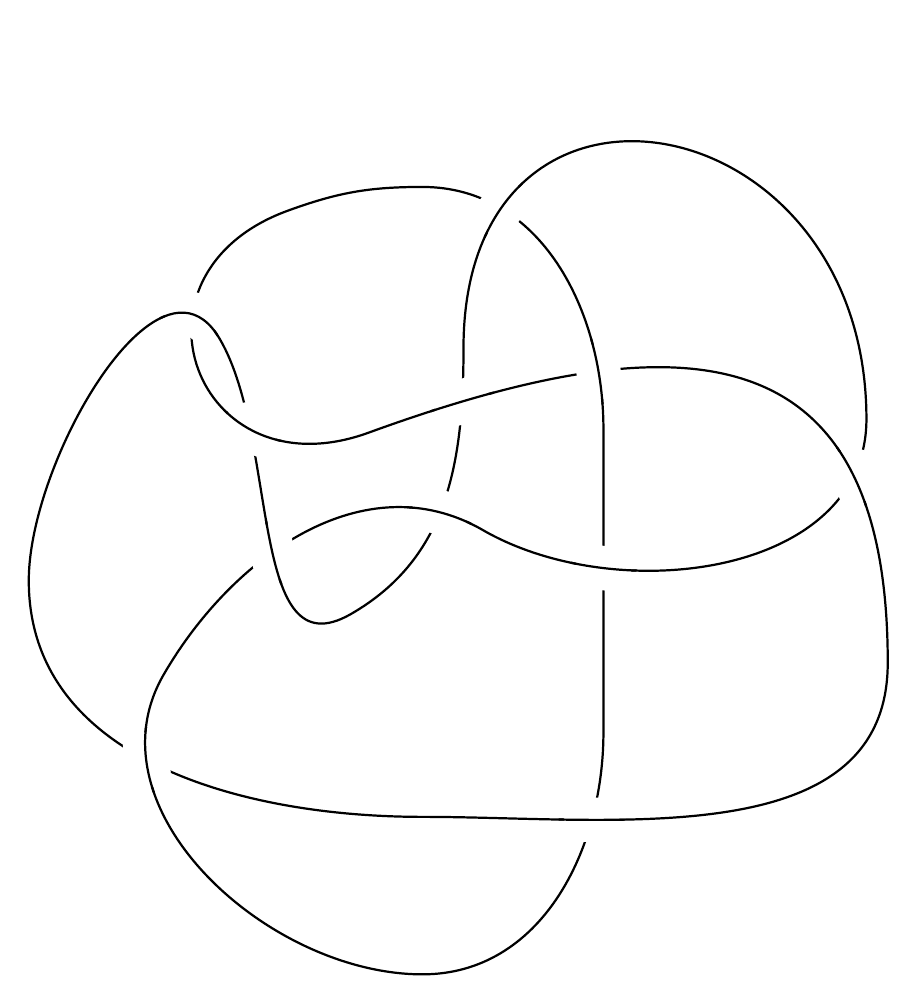
\begin{tikzpicture}
      \coordinate (a1) at (90:5);
      \coordinate (a2) at (40:3);
      \coordinate (a3) at (-40:3);
      \coordinate (a4) at (-90:5);
      \coordinate (a5) at (-160:3.5);
      \coordinate (a6) at (40:1);
      \coordinate (a7) at (20:6);
      \coordinate (a8) at (80:3);
      \coordinate (a9) at (180+25:1);
      \coordinate (a10) at (130:4);
      \coordinate (a11) at (180:5);
      \coordinate (a12) at (-90:3);
      \coordinate (a13) at (-10:6);
      \coordinate (a14) at (110:2);
      \coordinate (a15) at (110:5);

      % \foreach \i in {1,..., 15} \fill (a\i) circle (5pt);

      \begin{knot}[
        consider self intersections, 
        clip width = 20pt, 
        % draft mode=crossings, 
        flip crossing=1, 
        flip crossing=3, 
        flip crossing=8, 
        flip crossing=4, 
        flip crossing=7, 
        flip crossing=10, 
        flip crossing=9
        ]
        \strand[thick] (a1) to[out=0, in=90] 
        (a2) to[out=-90, in=90] 
        (a3) to[out=-90, in=0] 
        (a4) to[out=180, in=-120]
        (a5) to[out=60, in=150]
        (a6) to[out=-30, in=-90] 
        (a7) to[out=90, in=90, looseness=2] 
        (a8) to[out=-90, in=30]
        (a9) to[out=-150, in=-60]
        (a10) to[out=120, in=90] 
        (a11) to[out=-90, in=180]
        (a12) to[out=0, in=-90] 
        (a13) to[out=90, in=20, looseness=1.5]
        (a14) to[out=-160, in=200, looseness=2]
        (a15) to[out=20, in=180] 
        (a1);
      \end{knot}
    \end{tikzpicture}
  }\bigskip

  \scalebox{.7}{
      $$\begin{bmatrix}1-t+t^2 & 0 \\ 0 & -t^{-1}+4-5t+4t^2-t^3\end{bmatrix}$$
    }
    % \caption{A diagram for knot $K11n164$.\label{k11n164 diagram}}
  \end{figure}

\end{columns}

  \end{frame}

  \begin{frame}{}

      Co więcej, macierz ta niesie tę samą informację, co macierz Alexandera $A_D$, tzn. 
    % przypisanego diagramowi $D$ ma tę samą zredukowaną postać normalną Smitha co macierz Alexandera, tzn.
    $$\ker(A_D)\cong \ker(D\phi)$$
    oraz 
    $$\coker(A_D)\oplus \Z[\Z]\cong\coker(D\phi).$$

  \end{frame}

 
  \begin{frame}{Bibliografia}
    \nocite{*}
    \bibliographystyle{amsalpha}
    \bibliography{lit.bib}
% \printbibliography
  \end{frame}

\end{document}
